\documentclass[12pt]{article}
\usepackage[utf8]{inputenc}
\usepackage{hyperref}
\usepackage{graphicx}
\usepackage{amsmath}
\usepackage{listings}
\usepackage{xcolor}
\usepackage{geometry}
\usepackage{enumitem}

% Define Solidity language for listings
\lstdefinelanguage{Solidity}{
  keywords={
    function, public, private, contract, address, mapping, struct, modifier,
    if, else, for, while, do, break, continue, return, returns, true, false,
    new, delete, uint, uint256, string, bool, bytes, bytes32, internal, storage,
    memory, payable, view, pure, constant, anonymous, indexed, interface
  },
  sensitive=true,
  comment=[l]{//},
  morecomment=[s]{/*}{*/},
  string=[b]",
  morestring=[b]'
}

% Set default listing style
\lstset{
  frame=single,
  breaklines=true,
  basicstyle=\ttfamily\small,
  keywordstyle=\color{blue}\bfseries,
  commentstyle=\color{green!60!black},
  stringstyle=\color{purple},
  numbers=left,
  numberstyle=\tiny,
  numbersep=5pt,
  showstringspaces=false,
  tabsize=2
}

\geometry{
    a4paper,
    margin=1in
}

\title{BuildFair: A Decentralized Protocol for Secure Construction Agreements -- Reducing Risk and Ensuring Fair Payments in Construction}
\author{Helena Boing, Sara Esteves, Florine Elskamp}
\date{\today}

\begin{document}

\maketitle

\begin{abstract}
BuildFair is a decentralized Ethereum protocol designed to address the challenges of trust and payment security in construction agreements, particularly within the European SME market. By leveraging smart contracts, BuildFair automates payment processes and ensures fair transactions while maintaining immutable records on the blockchain, mitigating risks of payment disputes and delays. This whitepaper presents the protocol's architecture, implementation details, and security considerations, with a focus on enhancing efficiency and transparency in construction projects for European SMEs.
\end{abstract}

\newpage

\tableofcontents

\newpage

\section{Introduction}
The European construction sector, a cornerstone of the European economy, faces persistent challenges, particularly for Small and Medium-sized Enterprises (SMEs). While representing a significant market opportunity (€840 billion serviceable available market\cite{nextmsc_analysis}), SMEs in construction often grapple with issues that hinder growth and efficiency. Among the most pressing are:

\begin{itemize}
    \item \textbf{Pervasive Payment Delays:} Late payments are a notorious problem in the construction industry, disproportionately impacting SME cash flow and financial stability. Industry reports indicate average payment delays of 60-90 days for European construction SMEs\cite{construction_standards}, severely straining their resources and ability to undertake new projects.
    \item \textbf{Lack of Trust and Transparency:} Construction projects often involve complex, multi-stage agreements and relationships between buyers and sellers. A lack of transparency in project progress and payment status can breed distrust, leading to disputes and inefficiencies\cite{european_market_report}.
    \item \textbf{Inefficient and Costly Dispute Resolution:} When disagreements arise regarding project scope, quality, or payment, traditional dispute resolution mechanisms are often slow, expensive, and adversarial. This process can be particularly damaging for SMEs with limited resources.
    \item \textbf{Complex and Fragmented Payment Processes:} The industry often relies on complex, multi-step payment structures that can be difficult to manage and track, leading to errors and delays.
    \item \textbf{Lack of Standardization:} The construction industry lacks standardized payment terms and procedures, leading to confusion and potential disputes.
\end{itemize}

These challenges are exacerbated by the industry's reliance on intermediaries, such as banks and financial institutions, which often impose high fees and strict regulations that can hinder SME growth and innovation.

\subsection{Introducing BuildFair}
BuildFair is a decentralized protocol built on the Ethereum blockchain that directly tackles these pain points. By leveraging the security and transparency of blockchain technology and the automation capabilities of smart contracts, BuildFair offers a revolutionary solution for creating, managing, and executing construction agreements.

\subsection{Core Value Proposition}
\begin{itemize}
    \item \textbf{Secure and Automated Payments:} Smart contracts automatically manage and release payments based on pre-defined project milestones or completion criteria, eliminating payment delays\cite{construction_standards} and ensuring fair compensation for sellers.
    \item \textbf{Enhanced Transparency and Trust:} All agreement terms, project milestones, and payment transactions are recorded immutably on the blockchain\cite{ethereum_yellow}, providing unparalleled transparency and building trust between buyers and sellers.
    \item \textbf{Increased Efficiency and Reduced Costs:} Automating contract management and payment processes minimizes administrative overhead, freeing up valuable time and resources\cite{european_market_report}.
    \item \textbf{Fair and Impartial Dispute Resolution:} Future development will include a decentralized jury system for efficient and impartial dispute resolution.
\end{itemize}

\section{Protocol Overview}
\subsection{Core Components}
BuildFair operates as a decentralized protocol comprised of three main components:

\begin{itemize}
    \item \textbf{Smart Contracts:} The heart of the BuildFair protocol resides in its suite of Ethereum smart contracts. These contracts define the logic for project creation, funding, milestone management, payment release, and role-based access control.
    \item \textbf{BuildFair Platform Interface (DApp):} A user-friendly web interface allows buyers and sellers to interact with the BuildFair protocol, managing projects and payments through interaction with the underlying smart contracts.
    \item \textbf{Ethereum Blockchain:} BuildFair is deployed on the Ethereum blockchain, leveraging its robust security, decentralization, and established ecosystem.
\end{itemize}

\subsection{Key Features}
\begin{itemize}
    \item \textbf{Decentralized and Trustless Agreements:} Eliminates intermediaries and central authorities, with agreements governed by code.
    \item \textbf{Automated Milestone-Based Payments:} Future enhancement to enable automatic payment release upon milestone completion.
    \item \textbf{Transparent and Immutable Records:} All project details and transactions are permanently recorded on the blockchain.
    \item \textbf{Role-Based Access Control:} Clear separation of buyer and seller permissions.
    \item \textbf{Secure Escrow Mechanism:} Project funds are held securely until work completion is verified.
\end{itemize}

\subsection{User Flows}
BuildFair is designed to streamline the agreement process for both buyers and sellers in construction projects. The core user flows are as follows:

\subsubsection{Project Creation Flow (Seller Initiated)}
\begin{enumerate}[label=\arabic*.]
    \item \textbf{Seller Initiates Project:} Using the BuildFair Platform, the Seller initiates a new project, specifying the Buyer's Ethereum address, the agreed-upon project amount (in ETH), and a detailed description of the project scope and terms.
    
    \item \textbf{Smart Contract Deployment:} The BuildFair platform interacts with the underlying smart contract to create a new Project instance on the blockchain, recording the project details and associating it with the specified Buyer and Seller addresses. The smart contract assigns a unique projectId to this new project.
    
    \item \textbf{Project Details Recorded:} All project details, including buyer and seller addresses, project amount, and description, are immutably recorded on the Ethereum blockchain within the newly created Project smart contract.
    
    \item \textbf{Project Creation Confirmation:} The Seller and Buyer receive confirmation of successful project creation through the BuildFair Platform.
\end{enumerate}

\subsubsection{Project Funding Flow (Buyer Initiated)}
\begin{enumerate}[label=\arabic*.]
    \item \textbf{Buyer Reviews Project Details:} The Buyer reviews the project details on the BuildFair Platform, ensuring they align with the agreed-upon terms.
    
    \item \textbf{Buyer Funds Project:} The Buyer uses the BuildFair Platform to initiate the funding process for the specific projectId. The platform guides the Buyer to deposit the exact agreed-upon ETH amount into the designated Project smart contract address.
    
    \item \textbf{Funds Secured in Escrow:} The deposited ETH is securely held in escrow within the Project smart contract. The contract verifies that the correct amount has been received and updates the project status to "Funded".
    
    \item \textbf{Funding Confirmation:} Both Buyer and Seller receive confirmation that the project has been successfully funded and that the funds are securely held in escrow.
\end{enumerate}

\subsubsection{Work Verification and Payment Release Flow (Buyer Initiated)}
\begin{enumerate}[label=\arabic*.]
    \item \textbf{Seller Completes Work (Off-Chain):} The Seller performs the agreed-upon construction work as per the project agreement, working off-chain.
    
    \item \textbf{Buyer Verifies Work Completion:} Upon project completion, the Buyer verifies that the work has been completed to their satisfaction, based on agreed-upon criteria (inspections, documentation, etc. – these verification methods are agreed upon off-chain as part of the project terms).
    
    \item \textbf{Buyer Initiates Payment Release:} If satisfied with the completed work, the Buyer uses the BuildFair Platform to initiate the payment release for the specific projectId.
    
    \item \textbf{Smart Contract Executes Payment Release:} The BuildFair platform triggers the endProject function in the Project smart contract. The smart contract verifies that the project is in the "Funded" state and then automatically releases the funds held in escrow to the Seller's Ethereum address. The project status is updated to "Ended".
    
    \item \textbf{Payment Confirmation:} Both Buyer and Seller receive confirmation of successful payment distribution through the BuildFair Platform.
\end{enumerate}

\begin{figure}[h]
    \centering
    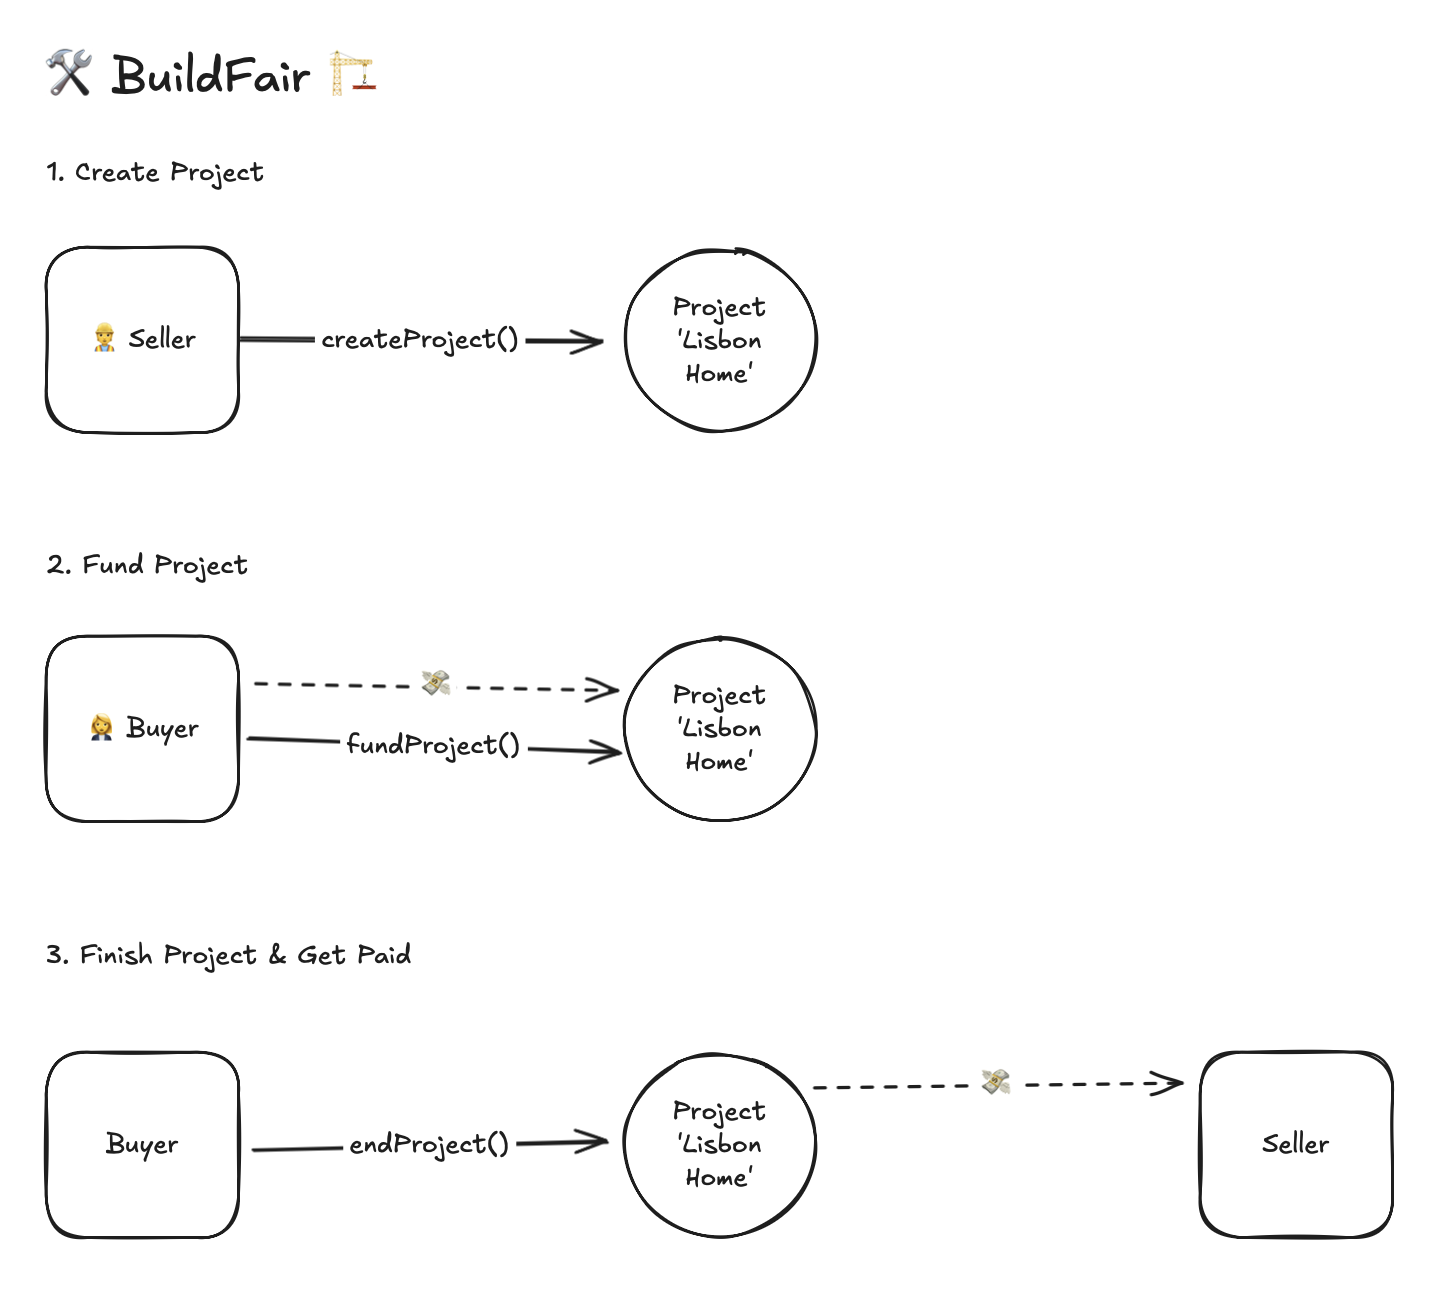
\includegraphics[width=\textwidth]{../buildfair-app/public/userflows.png}
    \caption{BuildFair User Interaction Flows}
    \label{fig:userflows}
\end{figure}

\section{Architecture}
\subsection{Smart Contract Design}
The BuildFair protocol's core logic is implemented through a set of robust and secure smart contracts written in Solidity, the primary smart contract language for Ethereum. These contracts are designed to be modular, auditable, and upgradeable where possible.

Key aspects of the smart contract design include:

\begin{itemize}
    \item \textbf{Project Contract:} This central smart contract manages the lifecycle of each construction project. It stores project details (buyer, seller, amount, description, status), enforces role-based access control, manages escrow functionality, and orchestrates payment release upon project completion.
    \item \textbf{Escrow Functionality:} The Project contract incorporates a secure escrow mechanism. When a project is funded, the Buyer's funds are transferred to and held securely within the Project contract itself. The funds remain locked in the contract until the endProject function is successfully executed by the Buyer after work verification.
    \item \textbf{State Management:} The contracts utilize a clear state management system (ProjectStatus enum) to track the different stages of a project (Created, Funded, Ended). State transitions are carefully controlled and verified within the smart contract functions to ensure predictable and secure contract behavior.
    \item \textbf{Custom Error Handling:} The smart contracts include custom error handling logic to provide informative error messages in case of failures or invalid operations. This enhances debugging and provides clearer feedback to users interacting with the protocol.
    \item \textbf{Gas Optimization:} Smart contract code is written with gas optimization principles in mind to minimize transaction costs for users interacting with the BuildFair protocol on the Ethereum network.
\end{itemize}

The BuildFair smart contracts are developed using industry-standard development tools such as Hardhat and are rigorously tested to ensure robustness and security. Prior to mainnet deployment, the smart contracts will undergo comprehensive security audits by reputable blockchain security firms to identify and mitigate any potential vulnerabilities.

\subsection{Role-Based Access Control}
BuildFair implements role-based access control within its smart contracts to ensure that only authorized parties can perform specific actions. The protocol defines two primary roles:

\subsubsection{Buyer}
\begin{itemize}
    \item \textbf{Permissions:} Buyers are authorized to fund projects by depositing ETH into the escrow, and to trigger payment release to the Seller upon verifying satisfactory work completion using the endProject function.
    \item \textbf{Responsibility:} Buyers are responsible for reviewing project details, funding the project according to the agreed amount, and verifying the completion of work before releasing payment.
\end{itemize}

\subsubsection{Seller}
\begin{itemize}
    \item \textbf{Permissions:} Sellers are authorized to initiate project creation using the createProject function, specifying project details. They are also entitled to receive payments from the escrow upon successful work verification and payment release by the Buyer.
    \item \textbf{Responsibility:} Sellers are responsible for initiating project creation with accurate details, performing the agreed-upon construction work off-chain, and ensuring project completion according to the agreed terms.
\end{itemize}

\section{Technical Implementation}
\subsection{Smart Contract Functions}
The following code illustrates the core smart contract functions of the BuildFair protocol, developed following industry best practices\cite{smart_contract_best}:

\begin{lstlisting}[language=Solidity]
// SPDX-License-Identifier: MIT
pragma solidity ^0.8.0;

enum ProjectStatus { Created, Funded, Ended }

contract BuildFairProject {
    struct Project {
        uint256 projectId;
        address buyer;
        address seller;
        uint256 amount;
        ProjectStatus status;
        string details;
    }

    mapping(uint256 => Project) public projects;
    uint256 public projectCounter;

    event ProjectCreated(uint256 projectId, address seller, address buyer, uint256 amount);
    event ProjectFunded(uint256 projectId, address buyer, uint256 amount);
    event ProjectEnded(uint256 projectId, address seller, uint256 amount);

    function createProject(address _buyer, uint256 _amount, string memory _details) 
        external returns (uint256) {
        projectCounter++;
        uint256 projectId = projectCounter;
        projects[projectId] = Project(
            projectId, _buyer, msg.sender, _amount, ProjectStatus.Created, _details
        );
        emit ProjectCreated(projectId, msg.sender, _buyer, _amount);
        return projectId;
    }

    function fundProject(uint256 _projectId) external payable {
        Project storage project = projects[_projectId];
        require(project.buyer == msg.sender, "Only buyer can fund project");
        require(project.status == ProjectStatus.Created, "Project must be in Created state");
        require(msg.value == project.amount, "Incorrect amount sent");

        payable(address(this)).transfer(msg.value);
        project.status = ProjectStatus.Funded;
        emit ProjectFunded(_projectId, msg.sender, msg.value);
    }

    function endProject(uint256 _projectId) external {
        Project storage project = projects[_projectId];
        require(project.buyer == msg.sender, "Only buyer can end project");
        require(project.status == ProjectStatus.Funded, "Project must be in Funded state");

        project.status = ProjectStatus.Ended;
        payable(project.seller).transfer(address(this).balance);
        emit ProjectEnded(_projectId, project.seller, project.amount);
    }

    function getProject(uint256 _projectId) external view returns (
        uint256 projectId,
        address buyer,
        address seller,
        uint256 amount,
        ProjectStatus status,
        string memory details
    ) {
        Project storage project = projects[_projectId];
        return (
            project.projectId,
            project.buyer,
            project.seller,
            project.amount,
            project.status,
            project.details
        );
    }
}
\end{lstlisting}

\subsection{Explanation of Key Functions}
The BuildFair smart contract implements several key functions that enable secure project management and payment automation:

\subsubsection{createProject Function}
\begin{lstlisting}[language=Solidity]
function createProject(address _buyer, uint256 _amount, string memory _details) 
    external returns (uint256)
\end{lstlisting}

\textbf{Purpose:} Allows a Seller to initiate a new construction project on the BuildFair protocol.

\textbf{Parameters:}
\begin{itemize}
    \item \texttt{\_buyer}: Ethereum address of the Buyer participating in the agreement
    \item \texttt{\_amount}: Agreed-upon project amount in Wei (smallest unit of ETH)
    \item \texttt{\_details}: String providing detailed project scope and terms
\end{itemize}

\textbf{Functionality:}
\begin{itemize}
    \item Increments \texttt{projectCounter} to generate a unique \texttt{projectId}
    \item Creates a new Project struct in the \texttt{projects} mapping
    \item Emits a \texttt{ProjectCreated} event with project details
    \item Returns the newly created \texttt{projectId}
\end{itemize}

\subsubsection{fundProject Function}
\begin{lstlisting}[language=Solidity]
function fundProject(uint256 _projectId) external payable
\end{lstlisting}

\textbf{Purpose:} Enables the Buyer to fund a project by depositing ETH into the smart contract escrow.

\textbf{Parameters:}
\begin{itemize}
    \item \texttt{\_projectId}: Unique identifier of the project to be funded
\end{itemize}

\textbf{Functionality:}
\begin{itemize}
    \item Retrieves Project struct using \texttt{\_projectId}
    \item Enforces role-based access control (only Buyer can fund)
    \item Verifies project state (must be in Created state)
    \item Validates sent amount matches agreed amount
    \item Transfers ETH to contract escrow
    \item Updates project status to Funded
    \item Emits \texttt{ProjectFunded} event
\end{itemize}

\subsubsection{endProject Function}
\begin{lstlisting}[language=Solidity]
function endProject(uint256 _projectId) external
\end{lstlisting}

\textbf{Purpose:} Allows Buyer to release escrowed funds to Seller upon project completion.

\textbf{Parameters:}
\begin{itemize}
    \item \texttt{\_projectId}: Unique identifier of the project to be ended
\end{itemize}

\textbf{Functionality:}
\begin{itemize}
    \item Retrieves Project struct using \texttt{\_projectId}
    \item Enforces role-based access control (only Buyer can end)
    \item Verifies project state (must be in Funded state)
    \item Updates project status to Ended
    \item Transfers escrowed funds to Seller's address
    \item Emits \texttt{ProjectEnded} event
\end{itemize}

\subsubsection{getProject Function}
\begin{lstlisting}[language=Solidity]
function getProject(uint256 _projectId) external view returns (...)
\end{lstlisting}

\textbf{Purpose:} Read-only function to retrieve project details.

\textbf{Parameters:}
\begin{itemize}
    \item \texttt{\_projectId}: Unique identifier of the project to retrieve
\end{itemize}

\textbf{Functionality:}
\begin{itemize}
    \item Retrieves and returns all Project struct fields
    \item Returns: projectId, buyer, seller, amount, status, details
\end{itemize}

\subsubsection{Data Structures}
The contract utilizes two primary data structures:

\textbf{Project Struct:}
\begin{itemize}
    \item \texttt{projectId} (uint256): Unique project identifier
    \item \texttt{buyer} (address): Buyer's Ethereum address
    \item \texttt{seller} (address): Seller's Ethereum address
    \item \texttt{amount} (uint256): Project amount in Wei
    \item \texttt{status} (ProjectStatus): Current project state
    \item \texttt{details} (string): Project specifications
\end{itemize}

\textbf{ProjectStatus Enum:}
\begin{itemize}
    \item Created: Initial state after project creation
    \item Funded: State after Buyer deposits funds
    \item Ended: Final state after payment release
\end{itemize}

\subsubsection{Key Logic Highlights}
\begin{itemize}
    \item \textbf{Event Emission:} Each core function emits events for blockchain logging and external system integration
    \item \textbf{Escrow Implementation:} Smart contract acts as trustless escrow, holding funds until work verification
    \item \textbf{Role and State Enforcement:} Strict access control and state transition verification ensure secure execution
\end{itemize}

\subsection{Project Lifecycle}
The BuildFair project lifecycle encompasses the following stages:

\begin{enumerate}
    \item \textbf{Project Creation (Seller Initiated):} The Seller initiates a new project through the BuildFair Platform, providing the Buyer's Ethereum address, project amount, and detailed project specifications. This action triggers the createProject smart contract function, deploying a new Project instance on the blockchain and recording the project's initial state as "Created."
    
    \item \textbf{Project Funding (Buyer Initiated):} Upon reviewing the project details, the Buyer funds the project by depositing the exact agreed-upon ETH amount into the Project smart contract address via the BuildFair Platform. This action invokes the fundProject smart contract function, which verifies the correct amount and updates the project status to "Funded," securing the funds in escrow.
    
    \item \textbf{Work Execution (Off-Chain):} The Seller performs the agreed-upon construction work off-chain, adhering to the project specifications and timelines agreed upon with the Buyer. BuildFair does not directly manage or monitor the off-chain work execution phase.
    
    \item \textbf{Work Verification (Buyer Initiated):} Once the Seller declares the project complete, the Buyer verifies the work based on pre-agreed criteria. This verification process occurs off-chain and is crucial for ensuring buyer satisfaction before payment release.
    
    \item \textbf{Payment Distribution (Buyer Initiated):} If the Buyer is satisfied with the completed work, they initiate payment release through the BuildFair Platform. This action calls the endProject smart contract function. The smart contract automatically releases the funds held in escrow to the Seller's Ethereum address and updates the project status to "Ended," completing the on-chain project lifecycle.
\end{enumerate}

\section{Security Considerations}
\subsection{Smart Contract Security}
BuildFair prioritizes security at every level of its design and implementation:

\begin{itemize}
    \item \textbf{Custom Error Handling:} BuildFair smart contracts employ custom error handling logic and informative error messages, providing clear feedback to users and developers when unexpected issues occur.
    
    \item \textbf{Role-Based Access Control:} Smart contract functions that modify contract state are protected by modifier checks, ensuring that only authorized users can execute critical functions.
    
    \item \textbf{State Transition Verification:} The contracts implement state transition verification to ensure that project lifecycles progress logically and predictably, preventing unexpected function calls in incorrect states.
    
    \item \textbf{Secure Fund Handling:} BuildFair utilizes a secure escrow mechanism where project funds are held directly within the Project smart contract, with carefully controlled fund transfers.
    
    \item \textbf{Reentrancy Protection:} The contracts are designed with reentrancy protection measures embedded in their state management logic, preventing potential recursive call exploits.
\end{itemize}

\subsection{Future Security Enhancements}
BuildFair is committed to continuous security improvement and plans to implement:

\begin{itemize}
    \item \textbf{Formal Verification:} Exploring formal verification techniques to mathematically prove the correctness and security properties of the smart contracts.
    
    \item \textbf{Decentralized Oracles:} For future features requiring integration with off-chain data sources, BuildFair will explore secure, decentralized oracles.
    
    \item \textbf{Continuous Monitoring:} Implementing continuous monitoring and vulnerability scanning tools for proactive security management.
    
    \item \textbf{Bug Bounty Program:} Establishing a public bug bounty program to incentivize security researchers to identify and responsibly disclose potential vulnerabilities.
\end{itemize}

\section{Economic Model}
BuildFair implements a sustainable economic model designed to ensure the long-term viability and continuous development of the protocol.

\subsection{Revenue Model}
BuildFair generates revenue through the following mechanisms:

\begin{itemize}
    \item \textbf{Transaction Fee:} A 2\% transaction fee is levied on each successful project transaction facilitated through the BuildFair protocol. This fee is calculated as 2\% of the project amount and is automatically deducted from the escrowed funds before payment release to the Seller. A minimum transaction fee of 0.01 ETH is applied to ensure economic viability for smaller transactions and cover gas costs associated with smart contract execution.
    
    The transaction fee is justified by the significant value BuildFair provides:
    \begin{itemize}
        \item Enhanced security and transparency
        \item Automation of payments
        \item Reduced risk of disputes
        \item Cost-effective compared to traditional project management
    \end{itemize}
    
    These fees fund ongoing protocol development, maintenance, security audits, community support, and platform infrastructure.
    
    \item \textbf{Subscription Plans (Future Feature):} Premium subscription plans targeted towards business users will unlock:
    \begin{itemize}
        \item Advanced project management tools
        \item Reporting dashboards
        \item API access with higher usage limits
        \item Dedicated support
    \end{itemize}
    
    \item \textbf{API Access (Future Feature):} Developer access to BuildFair infrastructure through tiered API pricing based on usage volume.
    
    \item \textbf{Smart Contract Deployment (Future Feature):} Custom smart contract deployment services for specialized construction agreements.
\end{itemize}

\subsection{Market Strategy}
BuildFair's initial market strategy focuses on penetrating the European construction market:

\begin{itemize}
    \item \textbf{Target Market:} SMEs and independent construction professionals, representing the backbone of the industry and facing acute challenges in payment security and contract management\cite{construction_standards}.
    
    \item \textbf{Initial Countries:} Focus on key European markets:
    \begin{itemize}
        \item Germany
        \item France
        \item Netherlands
        \item United Kingdom
    \end{itemize}
    These countries offer significant construction activity, high technological adoption, and established SME sectors\cite{european_market_report}.
    
    \item \textbf{Market Size:} €840 billion serviceable available market in European construction\cite{nextmsc_analysis}.
    
    \item \textbf{Growth Target:} 0.5-1\% market penetration within first 3-5 years of operation, establishing a strong foundation for future expansion.
\end{itemize}

\section{Future Development}
BuildFair is designed for continuous evolution and improvement. Future development efforts will focus on expanding functionality, enhancing user experience, and broadening the protocol's reach.

\subsection{Planned Features}
\begin{itemize}
    \item \textbf{Milestone-Based Payment System:}
    \begin{itemize}
        \item Automatic payment release upon milestone completion
        \item Enhanced verification mechanisms
        \item Flexible project structuring
        \item Improved risk mitigation
    \end{itemize}
    
    \item \textbf{Decentralized Jury System:}
    \begin{itemize}
        \item Network of impartial jurors
        \item Transparent dispute resolution
        \item Incentivized participation
        \item Cost-effective alternative to legal proceedings
    \end{itemize}
    
    \item \textbf{Enhanced Evidence Submission:}
    \begin{itemize}
        \item Secure document storage
        \item Blockchain-verified timestamps
        \item Multi-media support
        \item Automated verification processes
    \end{itemize}
    
    \item \textbf{Multi-Party Project Support:}
    \begin{itemize}
        \item Complex agreement structures
        \item Subcontractor integration
        \item Supply chain management
        \item Multi-stakeholder coordination
    \end{itemize}
    
    \item \textbf{Cross-Chain Compatibility:}
    \begin{itemize}
        \item Support for multiple blockchain networks
        \item Enhanced liquidity access
        \item Broader market reach
        \item Improved flexibility
    \end{itemize}
\end{itemize}

\subsection{Protocol Upgrades}
\begin{itemize}
    \item \textbf{Governance Implementation:}
    \begin{itemize}
        \item Decentralized decision-making
        \item Community-driven protocol evolution
        \item Token-based voting mechanisms
        \item Transparent upgrade processes
    \end{itemize}
    
    \item \textbf{Layer 2 Scaling Solutions:}
    \begin{itemize}
        \item Optimistic Rollups integration
        \item Reduced transaction costs
        \item Improved transaction speed
        \item Enhanced scalability
    \end{itemize}
    
    \item \textbf{Stablecoin Integration:}
    \begin{itemize}
        \item USDC and EUROC support
        \item Price stability for long-term projects
        \item Reduced volatility risk
        \item Enhanced user adoption
    \end{itemize}
    
    \item \textbf{Enhanced User Onboarding:}
    \begin{itemize}
        \item Simplified wallet management
        \item Educational resources
        \item Account abstraction
        \item Intuitive interfaces
    \end{itemize}
\end{itemize}

\section{Conclusion}
BuildFair represents a transformative advancement in modernizing construction agreements through blockchain technology. By providing a secure, transparent, and automated platform built on the Ethereum network, BuildFair directly addresses critical challenges plaguing the European SME construction market and beyond.

The protocol's key strengths include:
\begin{itemize}
    \item Robust smart contract architecture ensuring security and reliability
    \item Focus on user experience and accessibility
    \item Sustainable economic model supporting long-term growth
    \item Strategic focus on the European SME construction sector
    \item Commitment to continuous development and improvement
\end{itemize}

With its innovative approach to construction agreement management and strong foundation in blockchain technology, BuildFair is positioned to revolutionize how construction projects are executed, fostering a more transparent, efficient, and trustworthy future for the industry.

\section{References}
\begin{thebibliography}{9}
\bibitem{ethereum_yellow} Ethereum Foundation, ``Ethereum Yellow Paper,'' 2024.
\bibitem{smart_contract_best} OpenZeppelin, ``Smart Contract Security Best Practices,'' 2024.
\bibitem{construction_standards} European Construction Industry Federation, ``Construction Industry Payment Standards,'' 2023.
\bibitem{european_market_report} European Commission, ``European Construction Market Report,'' 2023.
\bibitem{nextmsc_analysis} NextMSC, ``Construction Market Analysis 2024-2030,'' 2024.
\end{thebibliography}

\end{document}